\documentclass[tikz]{standalone} 
\usepackage{xcolor}
\usepackage{pgfplots} 



\begin{document}
	\usetikzlibrary{dsp}
	\usetikzlibrary{chains}
	\usetikzlibrary{shapes.geometric}
	\usetikzlibrary{calc}
	


\pgfkeys{
    /prepare label/.style={
        /print label/\detokenize{#1}/.code={\ttfamily\detokenize{#1}}
    },
    /prepare label/.list={FCRN,FCRN15, gGCRN16, CRUSE, FDKF}
}

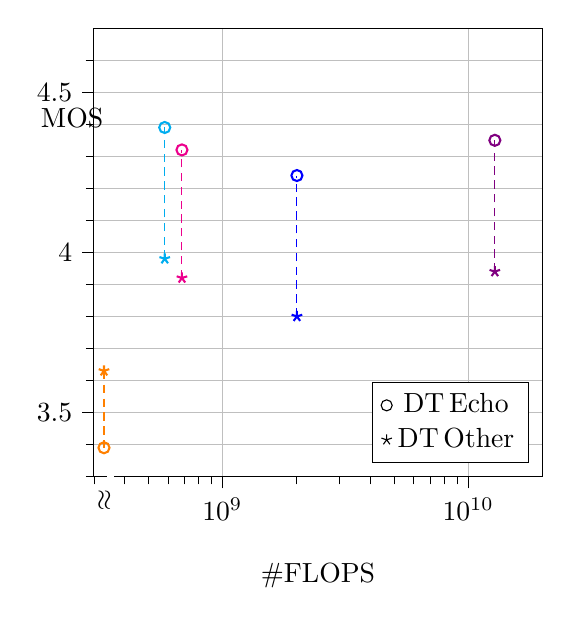
\begin{tikzpicture}

\begin{axis}[
width=.60*\columnwidth,
height=.60*\columnwidth,
legend cell align={left},
legend style={fill opacity=1.0, draw opacity=1, text opacity=1, draw=white!80!black},
log basis x={10},
tick align=outside,
tick pos=left,
xlabel={\#FLOPS},
% x labels style = {color=black}
xmajorgrids,
xmin=300000000, xmax=20000000000,
xmode=log,
tick style={color=black},
% y label style={anchor=north, xshift=0mm, font=\big},
y label style={anchor=north, xshift=17mm, yshift=-3mm},
% y label style={anchor=north, xshift=-22mm, yshift=-6mm},
ylabel={\rotatebox[origin=c]{270}{{MOS}}},
% ylabel={\rotatebox[origin=c]{270}{\raisebox{3mm}[4mm][2mm]{MOS}}},
ymajorgrids,
yminorgrids,
minor y tick num=4,
ymin=3.3, ymax=4.7,
extra y ticks={4.6},
extra y tick labels={
    {}
},
extra y tick style={%
    major tick length=3pt,
},
% ytick style={color=black},
extra x ticks={350000000},
extra x tick style={%
    every tick/.append style={white, line width=2.7pt},
    yshift=1pt,
    % every tick/.append style={red},
    grid=none,
},
extra x tick labels={
    {}
    % \rotatebox[origin=c]{270}{\rule{3mm}{$\approx$}}
},
]
\addplot[
        mark=star,
        line width=0.75pt,
        % mark size=6pt,
        only marks,
        point meta=explicit symbolic,
        violet,
        nodes near coords={
            \pgfkeys{/print label/\pgfplotspointmeta/.try}
        },
        every node near coord/.append style={font=\small, anchor=south,yshift=-13pt}
    ]
        table[header=false,meta index=0,x index=1,y index=2]{
			FCRN_ 12840000000 3.94
        };
\addplot[
        mark=star,
        line width=0.75pt,
        only marks,
        point meta=explicit symbolic,
        blue,
        nodes near coords={
            \pgfkeys{/print label/\pgfplotspointmeta/.try}
        },
        every node near coord/.append style={font=\small, anchor=south,yshift=-13pt, inner sep=2}
    ]
        table[header=false,meta index=0,x index=1,y index=2]{
			FCRN15_ 2011000000 3.80
        };
\addplot[
        mark=star,
        line width=0.75pt,
        only marks,
        point meta=explicit symbolic,
        cyan,
        nodes near coords={
            \pgfkeys{/print label/\pgfplotspointmeta/.try}
        },
        every node near coord/.append style={font=\small, anchor=south,yshift=-18pt, inner sep=2}
    ]
        table[header=false,meta index=0,x index=1,y index=2]{
			gGCRN16_ 583000000 3.98	
        };
\addplot[
        mark=star,
        line width=0.75pt,
        only marks,
        point meta=explicit symbolic,
        magenta,
        nodes near coords={
            \pgfkeys{/print label/\pgfplotspointmeta/.try}
        },
        every node near coord/.append style={font=\small, anchor=south,yshift=-13pt, inner sep=2}
    ]
        table[header=false,meta index=0,x index=1,y index=2]{
			CRUSE_ 685000000 3.92
        };
\addplot[
        mark=star,
        line width=0.75pt,
        only marks,
        point meta=explicit symbolic,
        orange,
        nodes near coords={
            \pgfkeys{/print label/\pgfplotspointmeta/.try}
        },
        every node near coord/.append style={font=\small, anchor=south,yshift=3.5pt, xshift=17pt, inner sep=2}
    ]
        table[header=false,meta index=0,x index=1,y index=2]{
			FDKF 330000000 3.63
        };
\end{axis}


\begin{axis}[
width=.60*\columnwidth,
height=.60*\columnwidth,
  axis y line*=right,
  axis x line=none,
xmin=300000000, xmax=20000000000,
xmode=log,
  ymin=3.3, ymax=4.7,
  % y axis line style=black,
% y label style={anchor=north, xshift=23mm, yshift=-81mm},
% ylabel={\rotatebox[origin=c]{270}{{MOS}}},
  %ylabel={DeltaSNR},
  every tick label/.append style={ticks=none, font=\big},
  legend pos=south east  
]
\addlegendimage{only marks, mark=o, black} \addlegendentry{DT\,Echo}
\addlegendimage{only marks, mark=star, black}\addlegendentry{DT\,Other}
\addplot[
        mark=o,
        line width=0.75pt,
        only marks,
        point meta=explicit symbolic,
        violet,
        nodes near coords={
            \pgfkeys{/print label/\pgfplotspointmeta/.try}
        },
        every node near coord/.append style={font=\small, anchor=south,yshift=+2pt, xshift=-1pt, inner sep=2}
    ]
        table[header=false,meta index=0,x index=1,y index=2]{
			FCRN 12840000000 4.35
        };
\addplot[
        mark=o,
        line width=0.75pt,
        only marks,
        point meta=explicit symbolic,
        blue,
        nodes near coords={
            \pgfkeys{/print label/\pgfplotspointmeta/.try}
        },
        every node near coord/.append style={font=\small, anchor=south,yshift=1pt}
    ]
        table[header=false,meta index=0,x index=1,y index=2]{
			FCRN15 2011000000 4.24
        };
\addplot[
        mark=o,
        line width=0.75pt,
        only marks,
        point meta=explicit symbolic,
        cyan,
        nodes near coords={
            \pgfkeys{/print label/\pgfplotspointmeta/.try}
        },
        every node near coord/.append style={font=\small, anchor=south,yshift=4.5pt, xshift=4pt}
    ]
        table[header=false,meta index=0,x index=1,y index=2]{
			gGCRN16 583000000 4.39	
        };
\addplot[
        mark=o,
        line width=0.75pt,
        only marks,
        point meta=explicit symbolic,
        magenta,
        nodes near coords={
            \pgfkeys{/print label/\pgfplotspointmeta/.try}
        },
        every node near coord/.append style={font=\small, anchor=south,yshift=3pt, xshift=+13pt}
    ]
        table[header=false,meta index=0,x index=1,y index=2]{
			CRUSE 685000000 4.32
        };
\addplot[
        mark=o,
        line width=0.75pt,
        only marks,
        point meta=explicit symbolic,
        orange,
        nodes near coords={
            \pgfkeys{/print label/\pgfplotspointmeta/.try}
        },
        every node near coord/.append style={font=\small, anchor=south,yshift=-14pt}
    ]
        table[header=false,meta index=0,x index=1,y index=2]{
			FDKF_ 330000000 3.39
        };


\draw [densely dashed, violet] (axis cs:12840000000,3.94) -- (axis cs:12840000000,4.35);
\draw [densely dashed, blue] (axis cs:2011000000,3.80) -- (axis cs:2011000000,4.24);
\draw [densely dashed, cyan] (axis cs:583000000,3.98) -- (axis cs:583000000,4.39); %gG
\draw [densely dashed, magenta] (axis cs:685000000,3.92) -- (axis cs:685000000,4.32);% Cruse
\draw [densely dashed, orange] (axis cs:330000000,3.63) -- (axis cs:330000000,3.39);% Kalman

\end{axis}

\draw (0.125,-0.15) node (t) {\rotatebox[origin=c]{270}{\rule{3mm}{0mm}{$\approx$}}};




\end{tikzpicture}



\end{document}
